\documentclass[border=4pt,12pt]{standalone}
% House style for redrawn exam diagrams (diagram-v4: 0.4pt lines, filled -latex arrows, fine dashes; stipple and hatching drawn as real dots/lines (no PDF/SVG patterns, so they render in every browser and at any scale); transparent background). Every figure \input's this.
\usepackage{amsmath,amssymb}
\usepackage{txfonts}
\usepackage{pdfrender,xcolor}
% \halo{text}: label on shading. The shading stops just around each letter's outline (a thin knock-out that follows the
% glyphs, like the papers' typesetting), never a box. Owner: "I don't want a box around the text".
\newcommand{\halo}[1]{\leavevmode\rlap{\pdfrender{TextRenderingMode=2,LineWidth=2.2pt,LineJoinStyle=1,StrokeColor=white,FillColor=white}#1}#1}
\usepackage{tikz,pgfplots}
\pgfplotsset{compat=1.18}
\usetikzlibrary{arrows.meta,calc,angles,quotes,patterns,patterns.meta,intersections,positioning,decorations.markings,shapes.geometric}
% Stipple and hatching are drawn as actual dots / lines clipped to the region (path picture), NOT as pattern fills:
% SVG <pattern> fills vanish or blur when browsers scale the image, so the owner could not see the shading.
% Each dot is a 0.72pt square (keeps SVGs small; reads as a dot at print size). Dots sit on one global staggered grid, so neighbouring regions line up.
\makeatletter
\newdimen\ex@x \newdimen\ex@y \newdimen\ex@xa \newdimen\ex@ya \newdimen\ex@xb \newdimen\ex@yb \newcount\ex@row
\def\exam@stipplecolor{black!75}\def\exam@dotr{0.42pt}\def\exam@dotgap{2.5}
\def\ex@rowdots{\ifdim\ex@x<\ex@xb \pgfpathrectangle{\pgfqpoint{\dimexpr\ex@x-0.36pt\relax}{\dimexpr\ex@y-0.36pt\relax}}{\pgfqpoint{0.72pt}{0.72pt}}\advance\ex@x by \exam@dotgap pt\relax\expandafter\ex@rowdots\fi}
\def\exam@stipple{%
  \pgftransformreset% dots are sized in real points even inside scaled pictures
  \pgfpointanchor{path picture bounding box}{south west}\ex@xa=\pgf@x \ex@ya=\pgf@y
  \pgfpointanchor{path picture bounding box}{north east}\ex@xb=\pgf@x \ex@yb=\pgf@y
  \pgfsetfillcolor{\exam@stipplecolor}\pgfmathsetmacro\ex@h{\exam@dotgap/2}%
  \pgfmathtruncatemacro\ex@r{floor(\ex@ya/\ex@h)-1}\ex@row=\ex@r\relax
  \ex@y=\ex@r\dimexpr\ex@h pt\relax
  \loop\ifdim\ex@y<\ex@yb
    \pgfmathtruncatemacro\ex@c{floor(\ex@xa/\exam@dotgap)-1}\ex@x=\ex@c\dimexpr\exam@dotgap pt\relax
    \ifodd\ex@row \advance\ex@x by \ex@h pt\fi
    \ex@rowdots
    \advance\ex@y by \ex@h pt \advance\ex@row by 1
    \ifnum\numexpr\ex@row-(\ex@row/4)*4\relax=0 \pgfusepath{fill}\fi% flush every 4 rows: bounded TeX memory, few clip copies in the SVG
  \repeat\pgfusepath{fill}}
\newdimen\ex@d
\def\exam@hatch#1{% #1 = 1 for /, -1 for \ ; lines 45 degrees, 3pt apart
  \pgftransformreset
  \pgfpointanchor{path picture bounding box}{south west}\ex@xa=\pgf@x \ex@ya=\pgf@y
  \pgfpointanchor{path picture bounding box}{north east}\ex@xb=\pgf@x \ex@yb=\pgf@y
  \ex@d=\dimexpr\ex@yb-\ex@ya\relax \ex@x=\dimexpr\ex@xa-\ex@d\relax
  \loop\ifdim\ex@x<\ex@xb
    \ifnum#1>0 \pgfpathmoveto{\pgfqpoint{\ex@x}{\ex@ya}}\pgfpathlineto{\pgfqpoint{\dimexpr\ex@x+\ex@d\relax}{\ex@yb}}%
    \else \pgfpathmoveto{\pgfqpoint{\ex@x}{\ex@yb}}\pgfpathlineto{\pgfqpoint{\dimexpr\ex@x+\ex@d\relax}{\ex@ya}}\fi
    \advance\ex@x by 4.24pt
  \repeat
  \pgfsetlinewidth{0.4pt}\pgfsetstrokecolor{black}\pgfusepath{stroke}}
\def\examstipple{\exam@stipple}\def\examhatch{\exam@hatch}\def\examsetstipplecolor#1{\def\exam@stipplecolor{#1}}\def\examsetdotgap#1{\def\exam@dotgap{#1}}
\makeatother
% (legacy pattern kept for old files)
% staggered stipple like the NESA papers' dotted shading
\pgfdeclarepatternformonly{exam stipple}{\pgfpointorigin}{\pgfqpoint{2.2pt}{2.2pt}}{\pgfqpoint{2.2pt}{2.2pt}}{%
  \pgfpathcircle{\pgfqpoint{0.55pt}{0.55pt}}{0.42pt}\pgfpathcircle{\pgfqpoint{1.65pt}{1.65pt}}{0.42pt}\pgfusepath{fill}}
\tikzset{
  every picture/.style={line width=0.6pt, >={Latex[length=2mm,width=1.3mm]}},
  curve/.style={line width=0.6pt},
  open arrow/.style={-{Latex[length=2mm,width=1.3mm]}},  % owner: filled -latex heads everywhere, no open chevrons
  aux/.style={dash pattern=on 2pt off 1.5pt, line width=0.6pt},
  shade/.code={\def\exA{#1}\def\exB{none}\ifx\exA\exB\else\pgfkeysalso{fill=black!18}\fi},
  shade/.default=on,
  shade dots/.style={fill=none, path picture={\examstipple}},
  stipple color/.code={\examsetstipplecolor{#1}},
  stipple gap/.code={\examsetdotgap{#1}},
  shade dense dots/.style={fill=none, stipple gap=1.6, path picture={\examstipple}},
  shade hatch/.style={fill=none, path picture={\examhatch{1}}},
  shade hatch reverse/.style={fill=none, path picture={\examhatch{-1}}},
  shade solid/.style={fill=black},
  pt/.style={circle, fill, inner sep=1.1pt},
  open pt/.style={circle, draw, fill=white, inner sep=1.1pt},
}
\pgfplotsset{
  exam axes/.style={axis lines=middle, axis line style={->}, xlabel={$x$}, ylabel={$y$},
    xlabel style={anchor=west}, ylabel style={anchor=south}, tick label style={font=\small},
    every axis plot/.append style={line width=0.6pt, black}, samples=200, clip=false,
    enlargelimits=false, axis on top},
}

\begin{document}
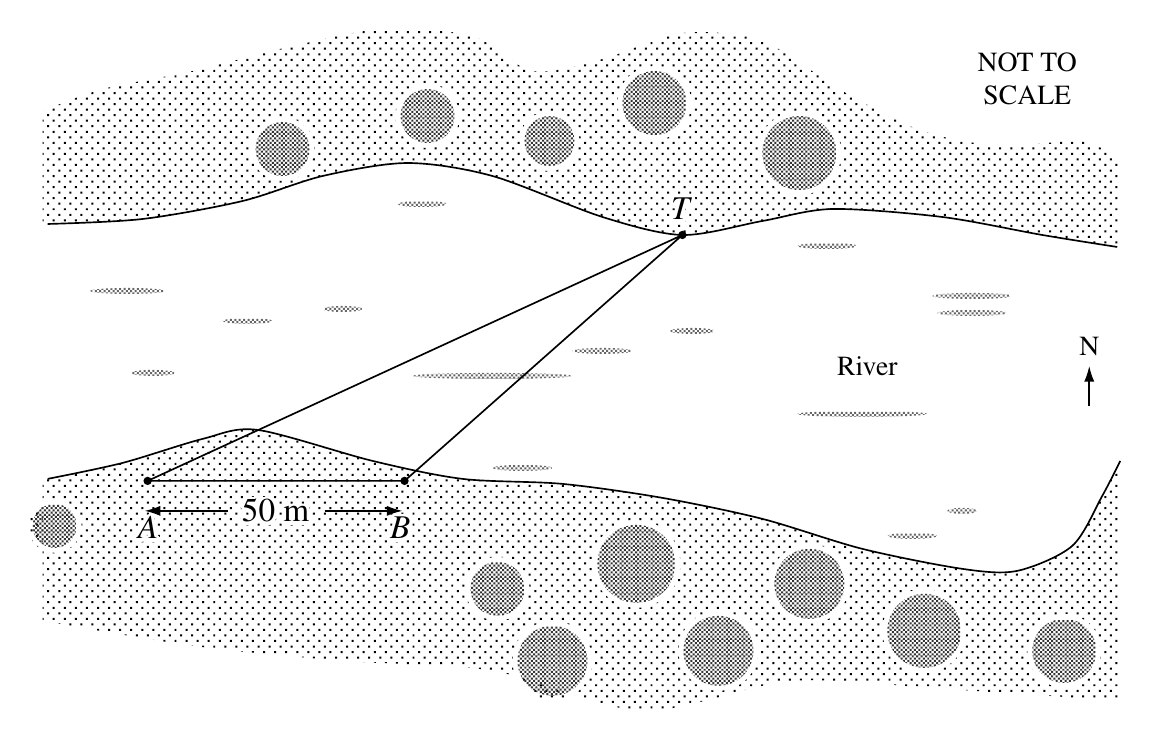
\begin{tikzpicture}[x=0.0127cm,y=-0.0127cm]
\def\upperedge{(5,203)(100,198)(200,180)(280,155)(365,142)(450,155)(560,196)(640,214)(720,200)(790,188)(900,196)(1000,214)(1075,226)}
\def\loweredge{(5,458)(80,442)(160,418)(215,409)(330,440)(420,458)(520,463)(620,477)(720,498)(820,528)(920,548)(975,550)(1030,525)(1060,475)(1078,440)}
% upper bank
\path[shade dots, stipple gap=4, stipple color=black, even odd rule]
  plot[smooth] coordinates {(0,90)(60,68)(150,50)(250,25)(340,8)(430,15)(490,50)(560,38)(640,12)(720,20)(800,70)(880,110)(960,125)(1040,120)(1078,140)}
  -- (1078,226) -- (1075,226) -- plot[smooth] coordinates {(1000,214)(900,196)(790,188)(720,200)(640,214)(560,196)(450,155)(365,142)(280,155)(200,180)(100,198)(5,203)} -- (0,203) -- cycle
  (240,128) circle[radius=32] (385,95) circle[radius=32] (507,120) circle[radius=30] (612,82) circle[radius=37] (757,132) circle[radius=42];
% lower bank
\path[shade dots, stipple gap=4, stipple color=black, even odd rule]
  (0,458) -- plot[smooth] coordinates \loweredge -- (1078,680)
  -- plot[smooth] coordinates {(1078,680)(900,668)(750,660)(600,690)(450,650)(300,640)(150,625)(0,600)} -- cycle
  (12,505) circle[radius=27] (455,568) circle[radius=32] (594,543) circle[radius=44] (510,640) circle[radius=40] (676,630) circle[radius=40] (767,563) circle[radius=40] (882,610) circle[radius=42] (1022,630) circle[radius=37];
% trees
\foreach \c/\r in {(240,128)/27,(385,95)/27,(507,120)/25,(612,82)/32,(757,132)/37,(12,505)/22,(455,568)/27,(594,543)/39,(510,640)/35,(676,630)/35,(767,563)/35,(882,610)/37,(1022,630)/32}
  \path[shade dense dots, stipple color=black!80] \c circle[radius=\r];
% ripples
\foreach \c/\w in {(380,183)/50,(85,270)/75,(300,288)/40,(205,300)/50,(110,352)/45,(450,355)/160,(560,330)/60,(650,310)/45,(785,225)/60,(930,275)/80,(930,292)/70,(820,393)/130,(480,447)/60,(870,515)/50,(920,490)/30}
  \path[shade dense dots, stipple color=black!60] \c ellipse[x radius=\w/2, y radius=3];
% river banks
\draw plot[smooth] coordinates \upperedge;
\draw plot[smooth] coordinates \loweredge;
% survey lines
\coordinate (A) at (105,460); \coordinate (B) at (362,460); \coordinate (T) at (640,214);
\draw (A)--(T) (B)--(T) (A)--(B);
\fill (A) circle[radius=1.5pt] (B) circle[radius=1.5pt] (T) circle[radius=1.5pt];
\node[font=\large] at (640,188) {\halo{$T$}};
\node[font=\large] at (105,507) {\halo{$A$}};
\node[font=\large] at (357,507) {\halo{$B$}};
\draw[<-] (102,490)--(185,490);
\draw[->] (282,490)--(360,490);
\node[font=\large] at (233,490) {\halo{50 m}};
% north, labels
\draw[->] (1047,385)--(1047,345);
\node at (1047,325) {N};
\node at (825,345) {River};
\node[align=center] at (985,58) {NOT TO\\SCALE};
\end{tikzpicture}
\end{document}